% !TEX root = thesis.tex
%%%%%%%%%%%%%%%%%%%%%%%%%%%%%%%%%%%%%%%%%%%%%%%%%%%%%%%%%%%%%%%%%%%%%%%%%%%%%%%
\chapter{Тестирование инструментальной среды}
\label{chap:testing}
%%%%%%%%%%%%%%%%%%%%%%%%%%%%%%%%%%%%%%%%%%%%%%%%%%%%%%%%%%%%%%%%%%%%%%%%%%%%%%%%

В данном разделе ставится задача проведения тестирования разработанной
программной системы на предмет наличия дефектов и соответствия функциональным
и нефункциональным требованиям.

\section{Функциональное тестирование}

Функциональное тестирование - это тестирование ПО в целях проверки реализуемости
функциональных требований. Для решения данной задачи необходимо протестировать
каждый элемент системы по отдельности и взаимодействие этих элементов в целом.
Так как метамодель лишь хранит данные и не содержит методы их обработки, ее
тестирование проводилось совместно с графическим интерфейсом и процедурами
анализа.

\subsection{Тестирование преобразователей}

Так как большая часть преобразователей - это код, сгенерированный при помощи
фреймворка ANTLR, модульное тестирование его функций не проводилось. Для
тестирования работоспособности использовался скрипт, запускающий соответствующий
преобразователь для разбора какой-либо системы. В качестве набора систем для
тестирования использовалось несколько десятков проектов с сайта github.com.
Правильность сериализованной модели проверялось при помощи графических средств
разработанной инструментальной среды (см. подразд.~\ref{subsec:graph_test}).

\subsection{Тестирование визуализации AST и CFG}
\label{subsec:graph_test}

В силу невозможности автоматизации проверки правильности отображения моделей и
метрик тестирование графического интерфейса проводилось вручную.

Алгоритм работы с системой выглядит следующим образом:

\begin{enumerate}
    \item Передача исходного кода анализируемой системы преобразователю для
    соответствующего языка программирования.
    \item Получение экземпляра метамодели и ее сериализация в формат XML.
    \item Десереализация и загрузка метамодели в инструментальную среду.
    \item Вызов процедур визуализации и анализа в ответ на действия пользователя.
\end{enumerate}

Для тестирования графического интерфейса был разработан набор небольших программ
для отображения основных конструкций языка. Ниже приведено несколько этапов
протокола испытаний:

\subsubsection{Тест №1}

Данный тест предназначен для проверки визуализации оператора условного ветвления.
Исходный код программы:

\begin{lstlisting}[caption={Тестовая программа}]
class Condition {
    public static void main(String[] args) {
        boolean learning = true;

        if (learning) {
            System.out.println("Java programmer");
        } else {
            System.out.println("What are you doing here?");
        }
    }
}
\end{lstlisting}

Визуализация графа потока управления. Как видно из рис.~\ref{fig:cfg_test1}
операция ветвления была отображена верно.

\newpage
\begin{figure}[h]
    \begin{center}
        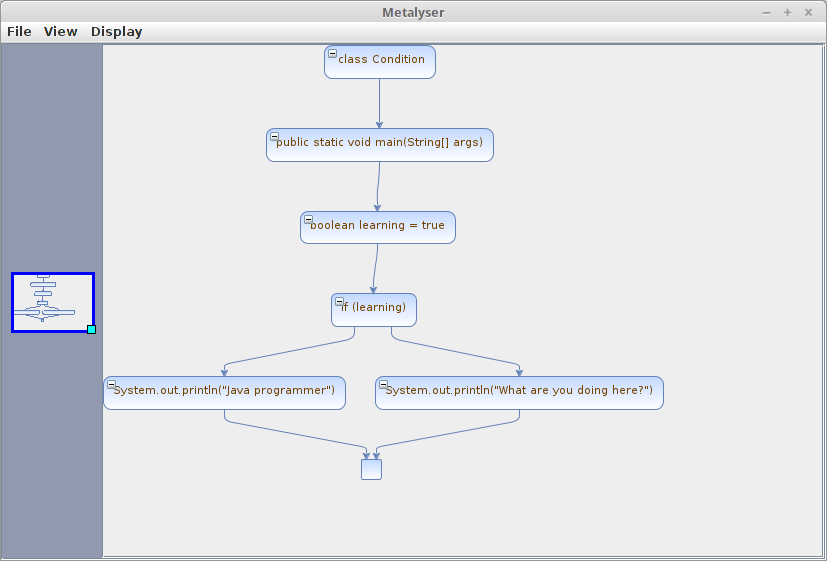
\includegraphics[width=0.7\textwidth]{cfg_test1.png}
    \end{center}
    \caption{Визуализация CFG тестового примера}
    \label{fig:cfg_test1}
\end{figure}

Визуализация абстрактного синтаксического дерева:

\begin{figure}[h]
    \begin{center}
        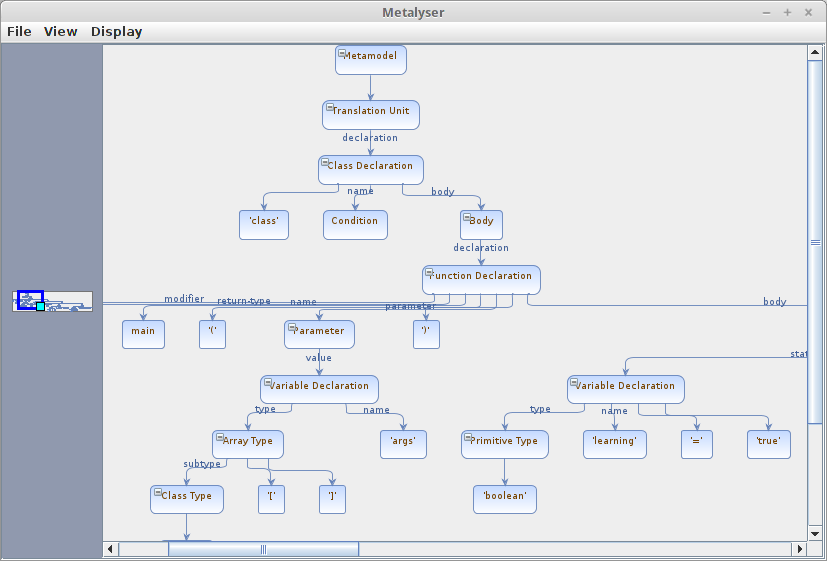
\includegraphics[width=0.75\textwidth]{ast_test1.png}
    \end{center}
    \caption{Визуализация AST тестового примера}
    \label{fig:ast_test1}
\end{figure}

\subsubsection{Тест №2}

Данный тест позволяет проверить правильность построения циклов. Исходный код
программы:

\begin{lstlisting}[caption={Тестовая программа}]
class Integers {
    public static void main(String[] arguments) {
        int c;
        for (c = 1; c <= 10; c++) {
          System.out.println(c);
        }
    }
}
\end{lstlisting}

Визуализация CFG:

\begin{figure}[h]
    \begin{center}
        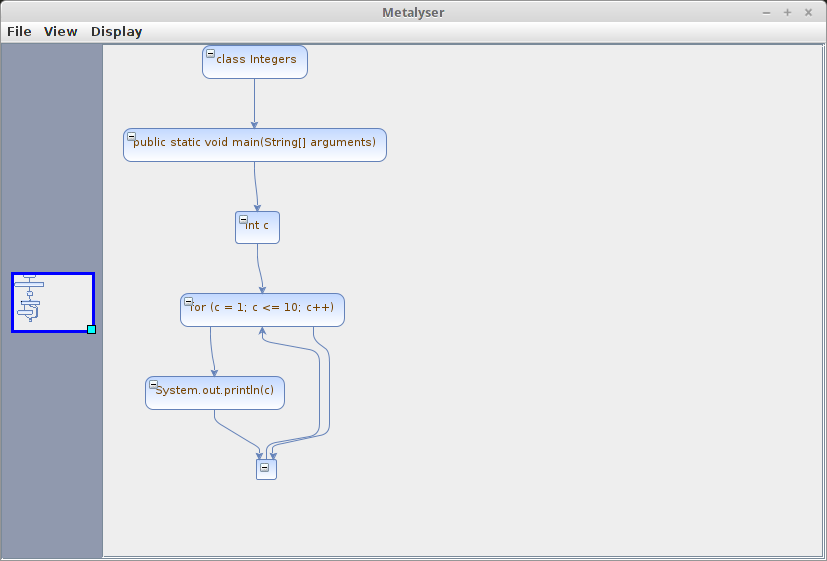
\includegraphics[width=\textwidth]{cfg_test2.png}
    \end{center}
    \caption{Визуализация CFG тестового примера}
    \label{fig:cfg_test2}
\end{figure}

Визуализация абстрактного синтаксического дерева:

\newpage
\begin{figure}[h]
    \begin{center}
        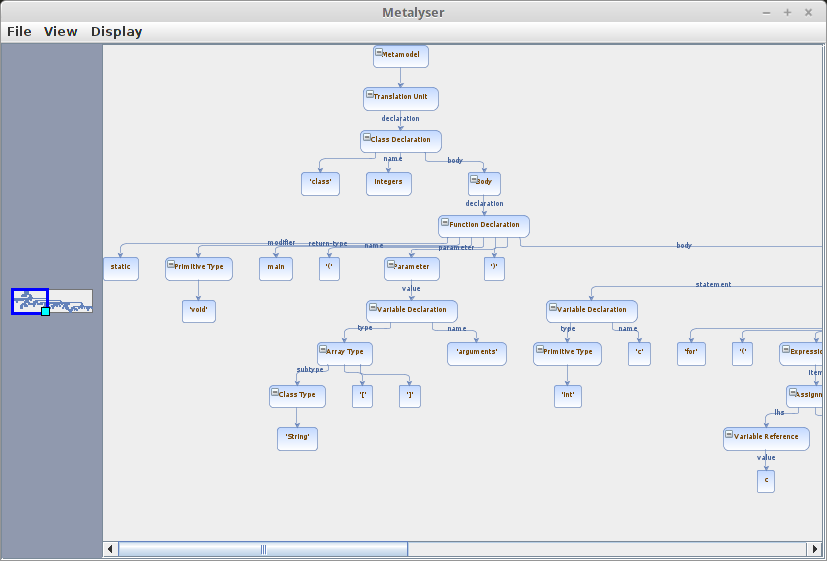
\includegraphics[width=\textwidth]{ast_test2.png}
    \end{center}
    \caption{Визуализация AST тестового примера}
    \label{fig:ast_test2}
\end{figure}

\subsection{Тестирование построения UML-диаграмм и метрик}

Для проверки правильно визуализации UML-диаграммы классов был разработан
следующий тестовый случай:

\begin{lstlisting}[caption={Тестовая программа}]
public class umlTest extends umlSuper {
    private final Test2 reference;
    private final Test3[] multipleReference;

    private int private1() {}
    private int private2() {}
    private int private3() {}

    public void public1() {}

    public static void main(final String[] args) {
        System.out.println("Hello, world!");
    }
}

class umlSuper {
    protected int x;
    public void public1() {}
    public void public2() {}
    public void public3() {}
}

class Test2 extends Super {
    private final int foo;
}

class Test3 extends Super {
    private final String bar;
}

class Super {
}
\end{lstlisting}

Соответствующая ему UML-диаграмма классов выглядит следующим образом:

\begin{figure}[h]
    \begin{center}
        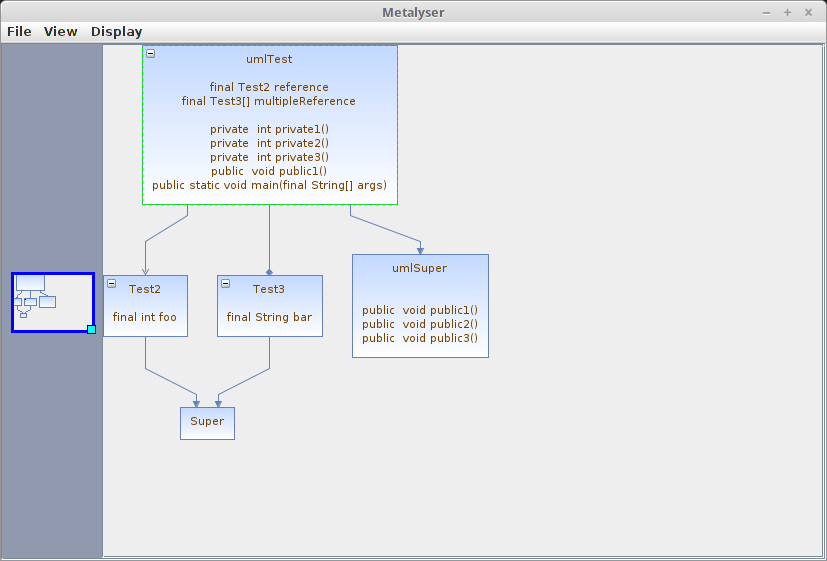
\includegraphics[width=\textwidth]{uml_test.png}
    \end{center}
    \caption{Диаграмма классов тестовой программы}
    \label{fig:uml_test}
\end{figure}
\newpage

Для класса \texttt{UmlTest} были получены следующие метрики:

\begin{figure}[h]
    \begin{center}
        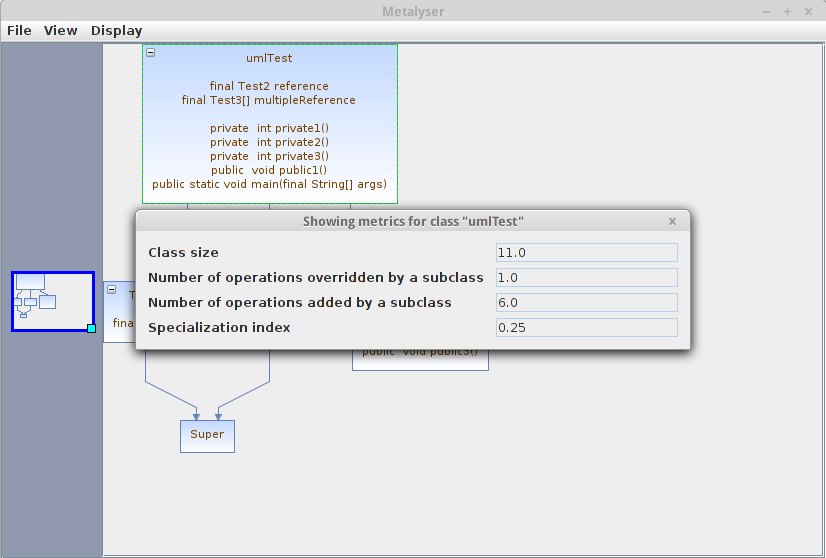
\includegraphics[width=\textwidth]{metrics_test.png}
    \end{center}
    \caption{Набор метрик Абреу для класса UmlTest}
    \label{fig:metrics_test}
\end{figure}

\section{Вывод}

Тестирование разработанной программной системы показало ее соответствие
сформулированным требованиям. Инструментальная среда позволяет извлекать и
визуализировать несколько моделей программ (CFG и AST), а также строить
UML-диаграммы классов и рассчитывать метрики Абреу для конкретного класса.
